\chapter{Estática de fluidos}	\label{hidrostatica}

\begin{miparrafo}
La materia ordinaria se presenta en alguno de los tres estados siguientes: sólido, líquido o gaseoso. Existe un cuarto estado de la materia denominado plasma que es esencialmente un gas ionizado.

Un sólido cristalino es aquél que tiene una estructura periódica y ordenada, como consecuencia, tiene una forma que no cambia, salvo por la acción de fuerzas externas. Cuando se aumenta la temperatura, los sólidos se funden y cambian al estado líquido. Las moléculas ya no permanecen en posiciones fijas, aunque las interacciones entre ellas sigue siendo suficientemente grande para que el líquido pueda cambiar de forma sin cambiar apreciablemente de volumen, adaptándose al recipiente que lo contiene.

En el estado gaseoso, las moléculas están en continuo movimiento y la interacción entre ellas es muy débil. Las interacciones tienen lugar, cuando las moléculas chocan entre sí. Un gas se adapta al recipiente que lo contiene pero trata de ocupar todo el espacio disponible.

En este capítulo, se estudiarán los denominados fluidos ideales o perfectos, aquellos que se pueden desplazar sin que presenten resistencia alguna	y que son incompresibles.
\end{miparrafo}

La \emph{hidrostática} es una parte de la \emph{hidrodinámica} que se encarga del estudio de los fluidos en reposo.

Fluido es aquella sustancia que es capaz de fluir: líquidos y gases. Los líquidos son mucho menos \emph{compresibles} que los gases, pero $\cdots$

\textbf{Primera hipótesis:} Supondremos que los fluidos son muy poco compresibles o no tienen compresibilidad.

Al rozamiento de los líquidos con los recipientes que los contienen se le llama \emph{viscosidad}, pero $\cdots$

\textbf{Segunda hipótesis:} Consideraremos que trabajamos con líquidos no viscosos, no rozan y por tanto no producen trabajo de rozamiento con las paredes de los recipientes que los contienen.

\section{Presión y densidad de un fluido}

Si en un sólido rígido aplicamos una fuerza, ésta se distribuye sobre toda su masa. En un gas libre no ocurre absolutamente nada. En la superficie libre y alejada de un líquido apenas se nota.

La solución a esto es la siguiente: si tenemos un fluido encerrado en un recipiente de modo que sus paredes o algunas de ellas pueden ser movidas por una fuerza exterior es la manera en que sí podemos notar la acción de la fuerza ejercida sobre el fluido.

\begin{multicols}{2}
Las fuerzas tangenciales provocan acciones tangenciales, esto es, acciones sobre las primeras moléculas más próximas a la superficie (tangentes). Como nuestros fluidos ideales son no viscosos, las acciones de las $\overrightarrow{F}_T$ no se transmitirán a todo el fluido.
\begin{figure}[H]
	\centering
	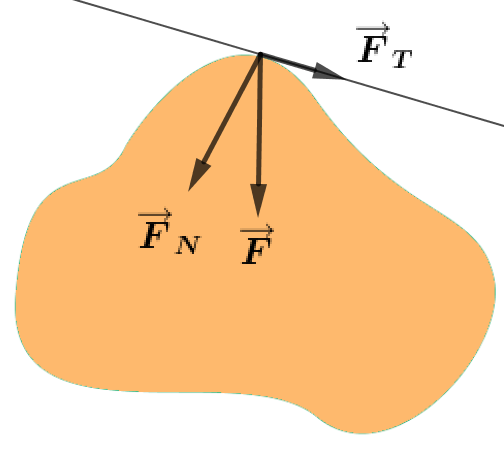
\includegraphics[width=.4\textwidth]{imagenes/imagenes07/T07IM01.png}
\end{figure}
\end{multicols}
La fuerza normal, $\overrightarrow{F}_N$, sí se transmite a toda la masa del fluido. Las fuerzas tangenciales no tendrán efecto, solo van a intervenir las fuerzas normales que nos van a introducir el concepto de \emph{presión}.

\begin{equation}
P=\lim_{S\to 0} \dfrac {F_N}{S}	
\end{equation}

Donde $S$ es la superficie y sus unidades en SI son $\mathrm{Nm^{-2}}$, también llamados \emph{Pascales}, $\mathrm{Pa}$. Sus dimensiones: $\ [\mathrm{P}]=[\mathrm{ML}^{-1}\mathrm{T}^{-2}]$.



\begin{multicols}{2}
$\quad$

Es frecuente representar la superficie en física por un vector, $\dd \overrightarrow{S}$, perpendicular al plano tangente a la superficie.
\begin{figure}[H]
	\centering
	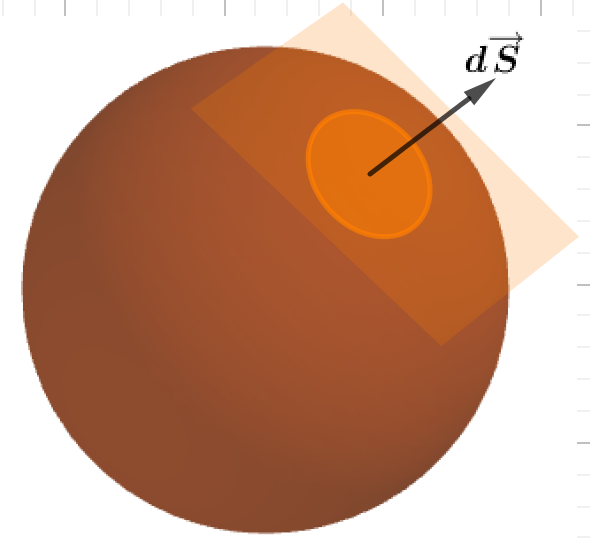
\includegraphics[width=.3\textwidth]{imagenes/imagenes07/T07IM02.png}
\end{figure}
\end{multicols}

Un elemento de superficie se puede representar por un vector $\dd \overrightarrow{S}$ que tiene por módulo es área geométrica de la superficie que representa y cuya dirección es normal a la superficie considerada y sentido hacia afuera de la misma.


Se define la densidad como:

\begin{equation}
\rho= \lim_{\Delta V \to 0}\dfrac{\Delta m}{\Delta V}=\dv{m}{V}	
\end{equation}

Unidades, $\ \mathrm{Kg\ m}^{-3}$ (en CGS\footnote{Sistema cegesimal de unidades: $\mathrm{cm,\ g,\ s}$}, se mide en $\mathrm{g \ cm}^{-3}$), dimensiones, $\ [\rho]=[\mathrm{ML}^{-3}]$.

\vspace{20mm} %**************************
\section{Variación de la presión en un fluido en reposo}
\begin{multicols}{2}
Un fluido está en reposo si, macroscópicamente, todas sus partículas están en reposo.

Consideremos un disco de fluido en reposo sometido a la acción del campo gravitatorio. Las fuerzas laterales a la misma altura $y$ del líquido en el disco de espesos $\dd y$ se conpensan (anulan) unas con otras.

Veamos que más fuerzas pueden intevenir.

\begin{figure}[H]
	\centering
	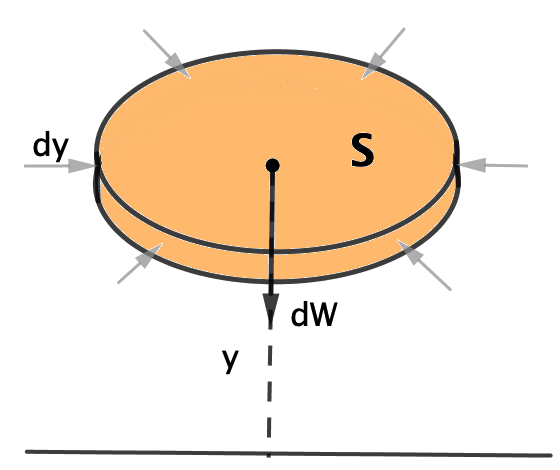
\includegraphics[width=.55\textwidth]{imagenes/imagenes07/T07IM03.png}
\end{figure}
\end{multicols}


Peso: $\ \dd W=g\ \dd m$

Por la parte de abajo del líquido la una presión es $P$, que dará lugar a una fuerza hacia arriba $P\cdot S$ \textcolor{gris}{(fuerza=presión x superficie)}.

Por encima del disco de fluido la presión es $P+\dd P$ cuya fuerza resultante hacia abajo es $(P+\dd P)\cdot S$ 

$\sum_i F_i=0 \to \quad g \ \dd m + (P+\dd P)\ S-P\ S=0 \to g\ \dd m +\dd P \ S=0$

$\dd m=\rho S\ \dd y \to \quad 0=g\ \rho \ \cancel{S} \ 
\dd y \ +\  \dd P \ \cancel{S} \to$

\begin{equation}
\label{ec.fdtal.hidrostatica}
\colorbox{LightYellow}{ \boxed{\boldsymbol{\ \dfrac{\dd P}{\dd y}=-\rho\ g\ }}}
\end{equation}
\emph{\textbf{Ecuación fundamental de la hidrostática}, da la variación de la presión con la altura.} La presión decrece al aumentar la altura (aumenta con la profundidad.)

Integrando:
$\quad \displaystyle \int_{P_1}^{P_2} \dd P=-\int_{y_1}^{y_2} \rho \ g\ \dd y \quad \to $


\begin{multicols}{2}
Integrando:

$\quad \displaystyle \int_{P_1}^{P_2} \dd P=-\int_{y_1}^{y_2} \rho \ g\ \dd y \quad \to $
\begin{equation}
P_2-P_1=-	 \int_{y_1}^{y_2} \rho \ g\ \dd y
\end{equation}
En los casos en que $\boldsymbol{ \rho, \ g}$ sean \textbf{constantes} ($\Delta y$ no demasiado grandes), con un cambio de notación:  

$P_2-P_1=\rho\ g \ (y_2-y_1)$

$y_2=y_1+h$

$P_1=P_0; \quad P_2=P  \Rightarrow$
\begin{equation}
\boxed{ \boldsymbol{ \ P=P_0+\rho \ g \ h \ }} 	
\end{equation}

\begin{figure}[H]
	\centering
	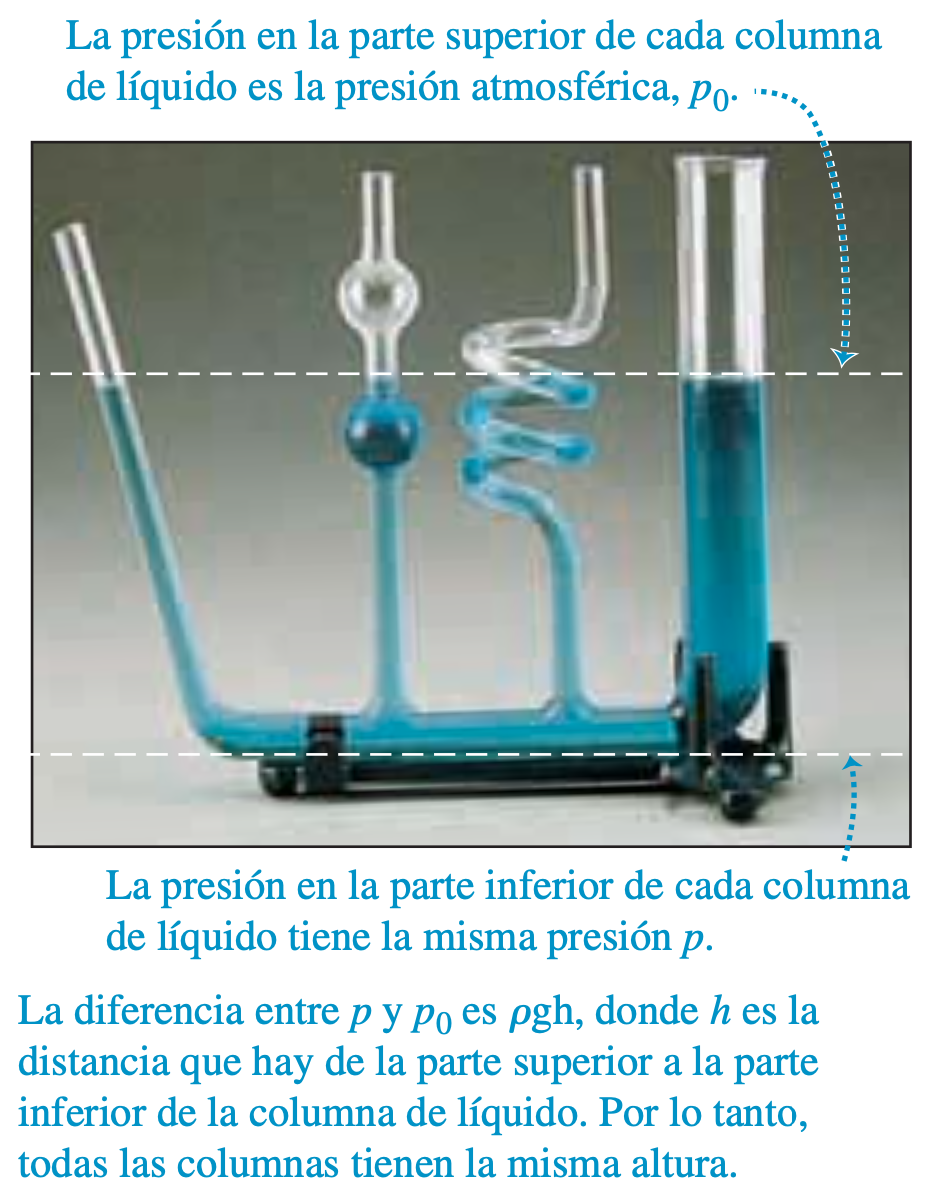
\includegraphics[width=.55\textwidth]{imagenes/imagenes07/T07IM14.png}
\end{figure}
\end{multicols}
\section{Ecuación barométrica}

\emph{Primera hipótesis: ``La atmósfera se comporta como un gas ideal''.} 

$PV=n R T=\dfrac m M T \to P= \dfrac m V \dfrac {RT}{M}=\rho \ \dfrac {RT}M \to \quad \rho=\dfrac M {RT}\ P$

De la ecuación fundamental de la hidrostática, tenemos que 

$\displaystyle \dfrac{\dd P}{\dd y}=-\rho\ g \to \quad \dfrac {\dd P}{\rho}=-g \ \dd y$, luego

$\dfrac{\dd P}{\dfrac {M}{RT} P}=-g \ \dd y \to \quad \dfrac {RT}M \ \dfrac {\dd P}P=-g\ \dd y \to \quad \displaystyle \int_{P_0}^P \dfrac {\dd P}P=-\dfrac {gM}{R} \int_0^y \dfrac{\dd y}{T}$

\emph{Segunda hipótesis: ``La temperatura no varía con la altura''.}

$\displaystyle \int_{P_0}^P \dfrac {\dd P}P=-\dfrac {gM}{RT} \int_0^y \dd y \to \quad \ln \dfrac P {P_0}=-\dfrac{gM}{RT}\ y$, despejando:

\begin{equation}
P=P_0\cdot e^{- \dfrac{gM}{RT}\ y}	
\end{equation}

\emph{Ecuación barométrica.} Indica como varía la presión con la altura a partir del nivel $0\ m$.

\underline{Inconvenientes}: el aire ni por aproximación es un gas ideal y la temperatura, incluso a pequeñas alturas, deja de ser constante con un poco de viento que sople.

\section{Manómetro y barómetro de Hg} 

\subsection{Manómetro}

En la base del tubo en U, la Presión a la izquierda ($P'\rho g x$)es igual a la presión en la parte derecha del tubo ($P_0+\rho g (x+h)$): 

La presión $P$ del recinto que queremos medir es

$P+\rho g x=P_o+\rho g (x+h) \qquad $
$\boldsymbol{P=P_0+\rho g h}$



\begin{figure}[H]
	\centering
	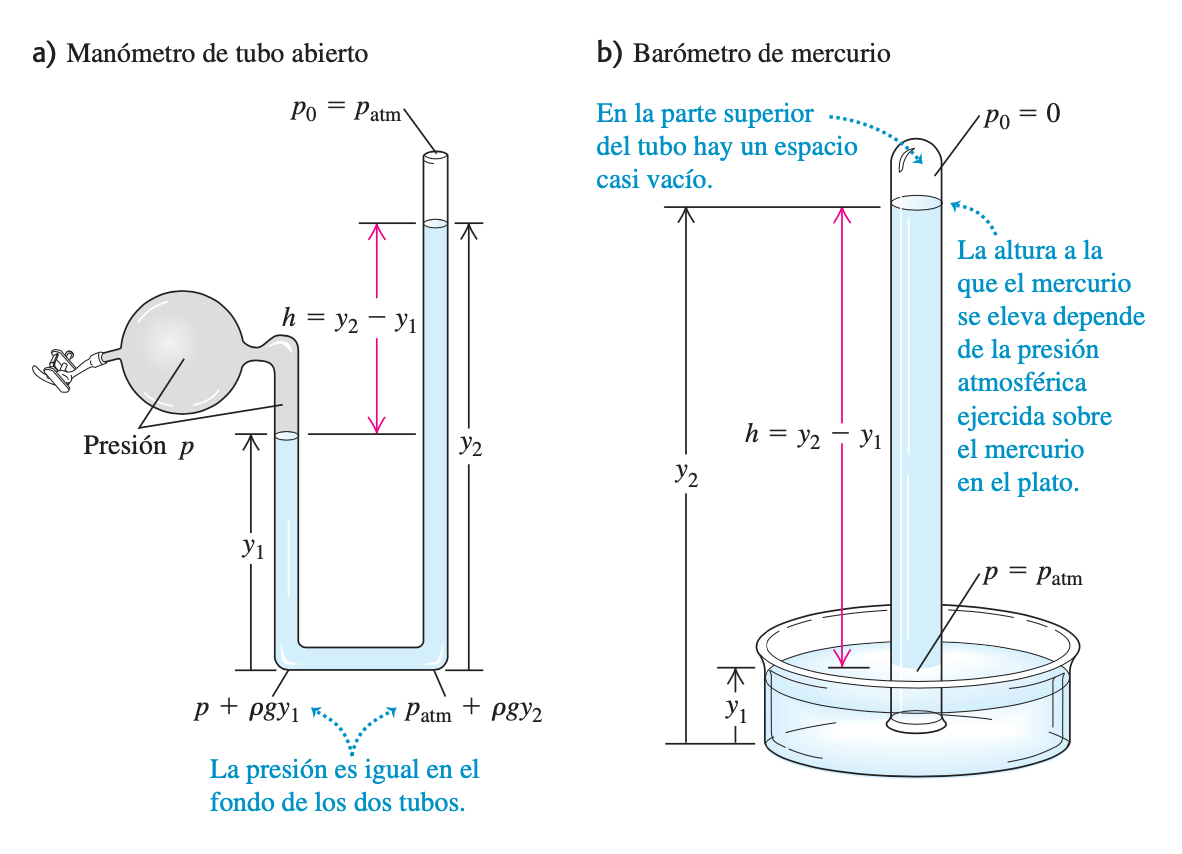
\includegraphics[width=1\textwidth]{imagenes/imagenes07/T07IM17.png}
\end{figure}



\subsection{Barómetro}

Se usa para determinar la presión atmosférica.

Por la forma de llenado, en la parte superior del tuvo se ha hecho el vacío, la presión en este punto es cero.

De nuevo igualamos la presión en la base a la parte izquierda del tubo, $P_0+\rho g x$, con la que hay en la parte derecha del mismo (estamos con la hipótesis de que nuestros fluidos son incompresibles):

$P_0+\rho g x=\rho g (x+h) \qquad \to \qquad $
$\boldsymbol{P_0=\rho g h}$

En el barómetro, la diferencia de alturas de las columnas de Hg nos da la medida de la presión atmosférica.


\begin{miparrafo}
El \textbf{experimento de Torricelli}  fue un proyecto realizado en 1643 por el físico y químico italiano Evangelista Torricelli en un laboratorio en el que logró medir la presión atmosférica por primera vez.

Torricelli, llenó con mercurio un tubo de 1 metro (100 cm) de largo, cerrado por uno de los extremos y lo invirtió sobre una cubeta llena de mercurio, de inmediato la columna de mercurio bajó varios centímetros, permaneciendo estática a unos 76 cm (760 mm) de altura. Este cambio en la altura de la columna de mercurio era causado por la atmosférica. Debido a que la presión es directamente proporcional a la altura de la columna de mercurio (Hg), así se adoptó como medida de la presión el mm (milímetro) de mercurio.

Torricelli llegó a la conclusión de que la columna de mercurio descendía debido a que la presión atmosférica ejercida sobre la superficie del mercurio era capaz de equilibrar la presión ejercida por ambos PESOS.

Otas unidades para la presión:

$\quad 760 \mathrm{mm}\ Hg = 1 \mathrm{atm}=1013.25 \ \mathrm{mbares}=101325 \ \mathrm{Pa}$ 

$\quad (1 \ \mathrm{bar}=10^3 \ \mathrm{mbares}=100 \ \mathrm{kPa})$
\end{miparrafo}

\section{Principio de Pascal}

En física, el principio de Pascal o ley de Pascal, es una ley 
enunciada por el físico-matemático francés Blaise Pascal (1623-1662) 
que se resume en la frase: \emph{``la presión ejercida sobre un fluido 
incompresible y en equilibrio dentro de un recipiente de paredes indeformables se 
transmite con igual intensidad en todas las direcciones y en todos los 
puntos del fluido''}.

En pocas palabras, se podría resumir afirmando que toda presión 
ejercida hacia un fluido, se propagará sobre toda la sustancia de 
manera uniforme. 
\begin{multicols}{2}
El principio de Pascal puede comprobarse utilizando una esfera hueca, perforada en diferentes lugares y provista de un émbolo. Al llenar la esfera con agua y ejercer presión sobre ella mediante el émbolo, se observa que el agua sale por todos los agujeros con la misma velocidad y por lo tanto con la misma presión.
\begin{figure}[H]
	\centering
	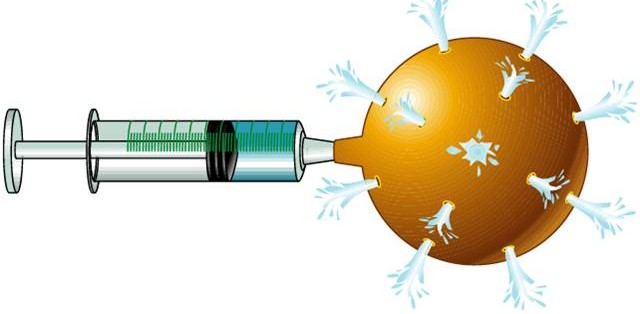
\includegraphics[width=.4\textwidth]{imagenes/imagenes07/T07IM06.png}
\end{figure}
\end{multicols}
También podemos observar aplicaciones del principio de Pascal en las prensas hidráulicas, en los elevadores hidráulicos, en los frenos hidráulicos, en los puentes hidráulicos y en los gatos hidráulicos.

\begin{figure}[H]
	\centering
	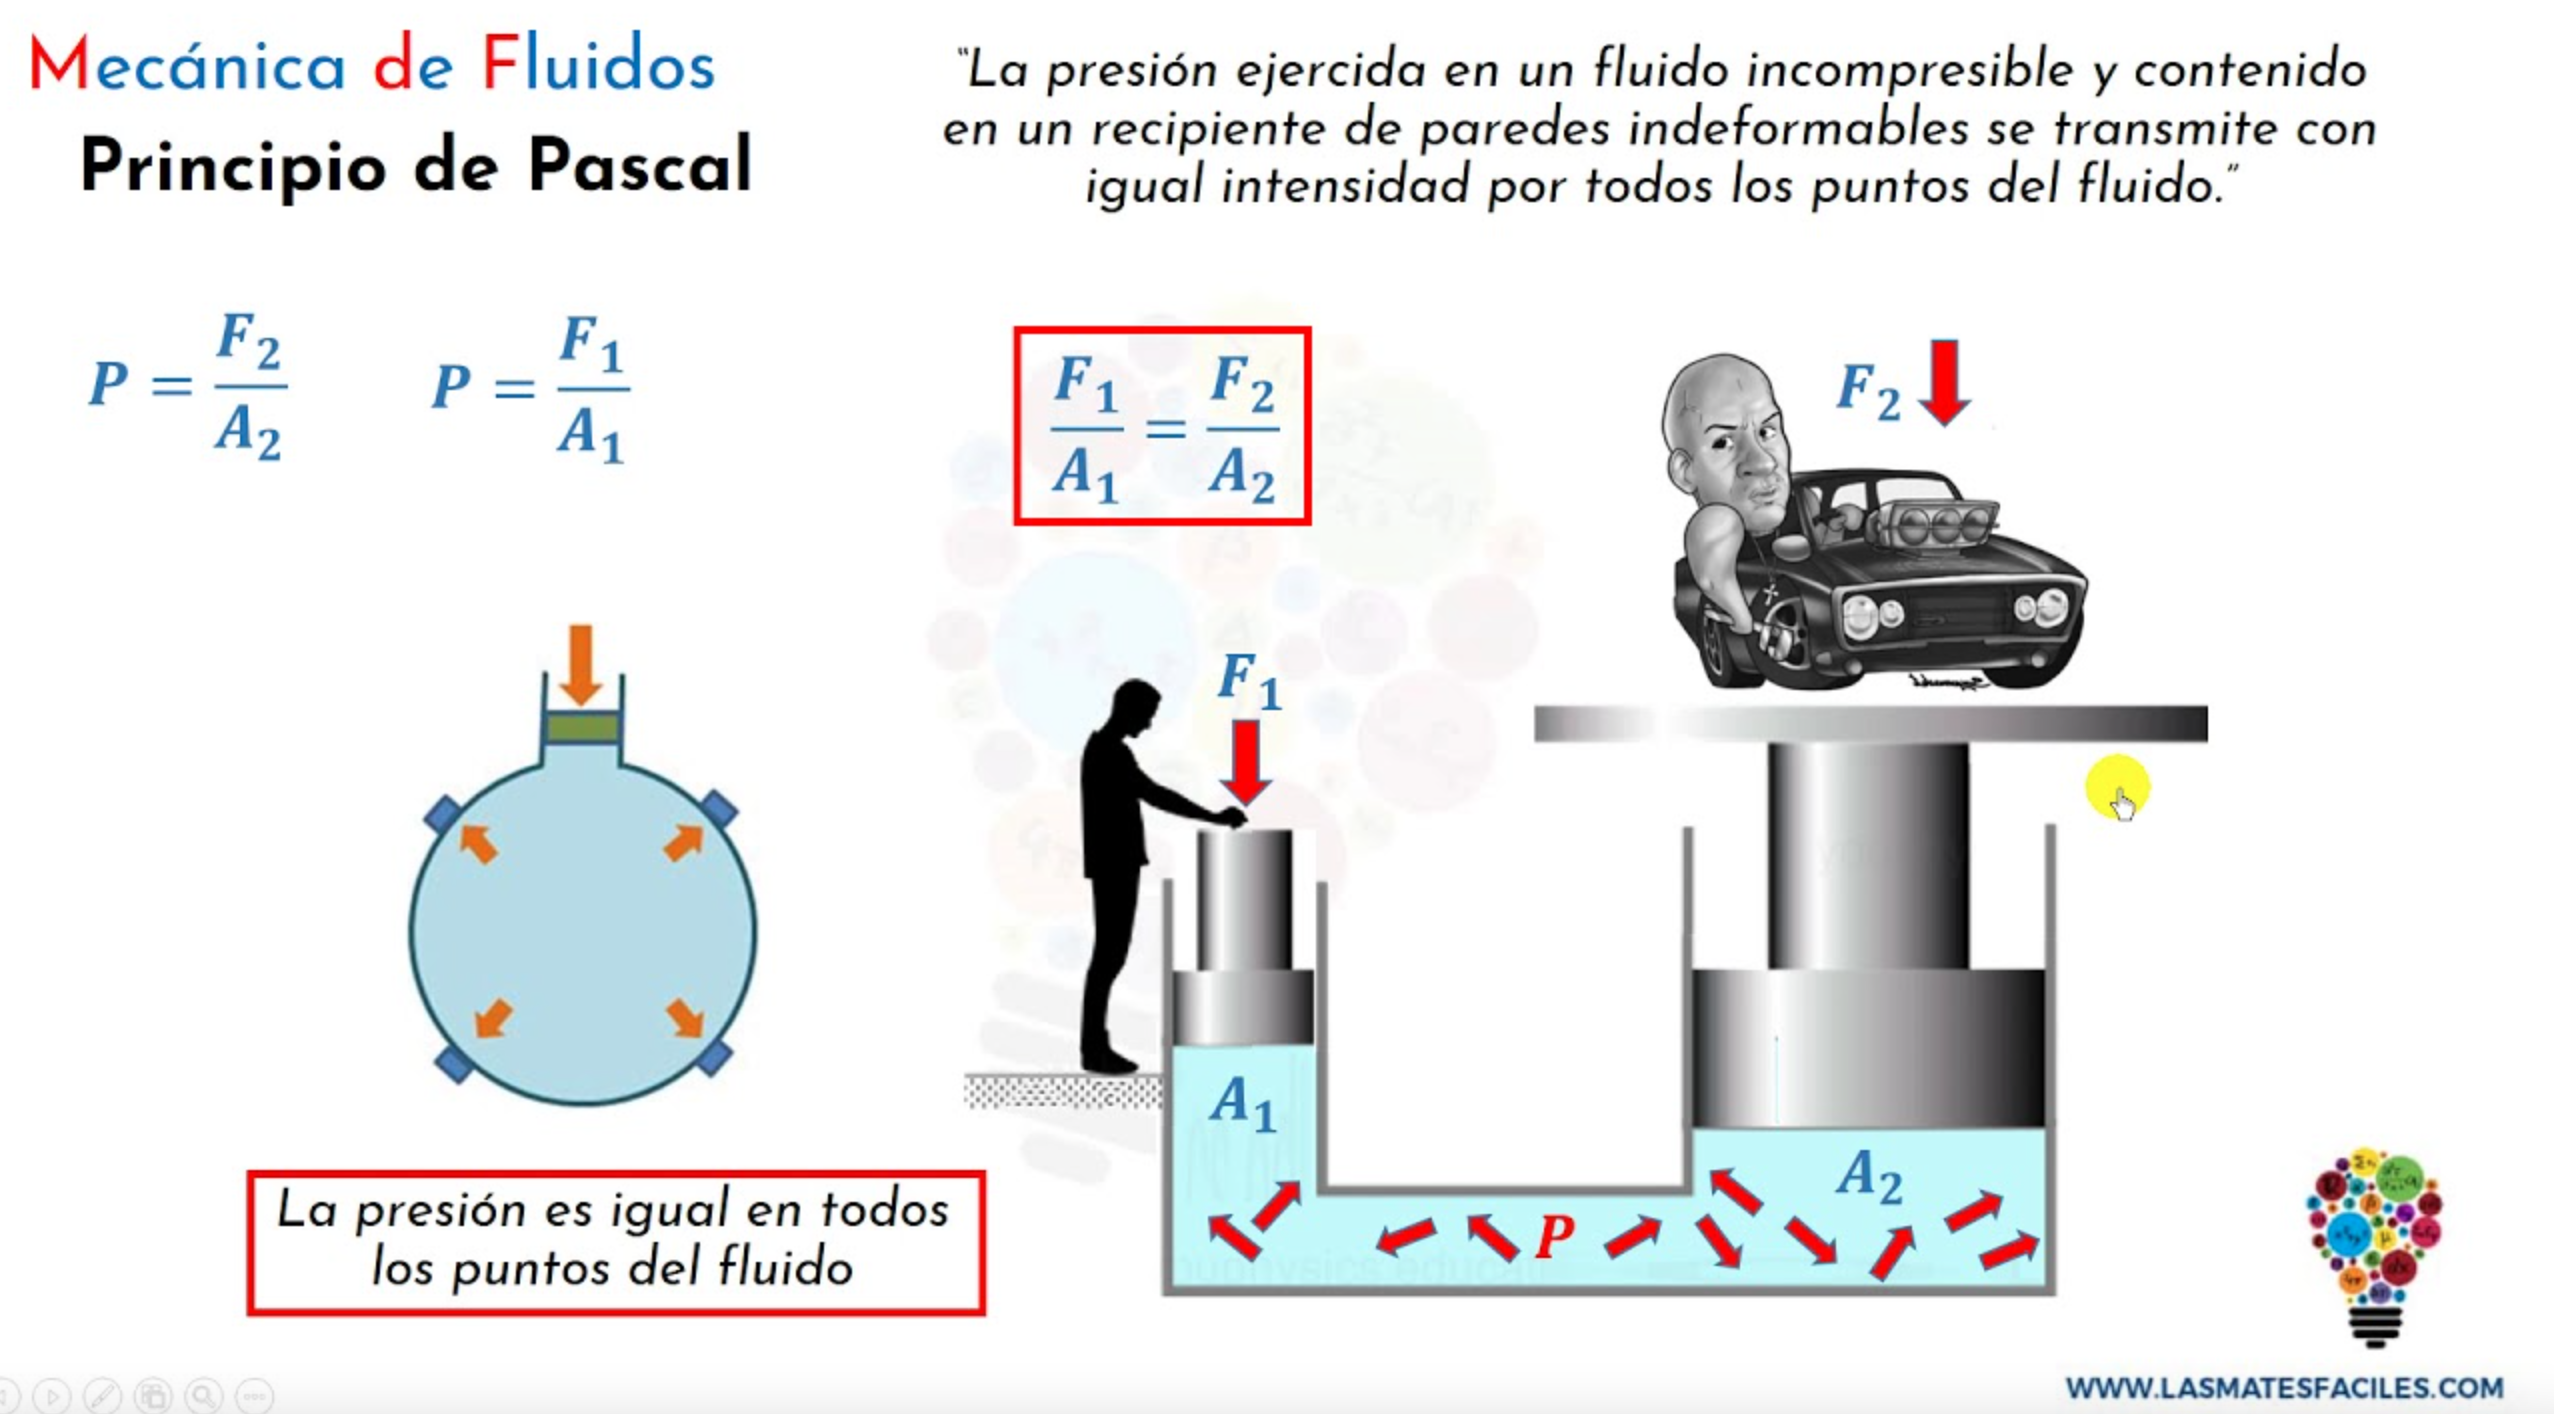
\includegraphics[width=1\textwidth]{imagenes/imagenes07/T07IM07.png}
\end{figure}

\begin{figure}[H]
	\centering
	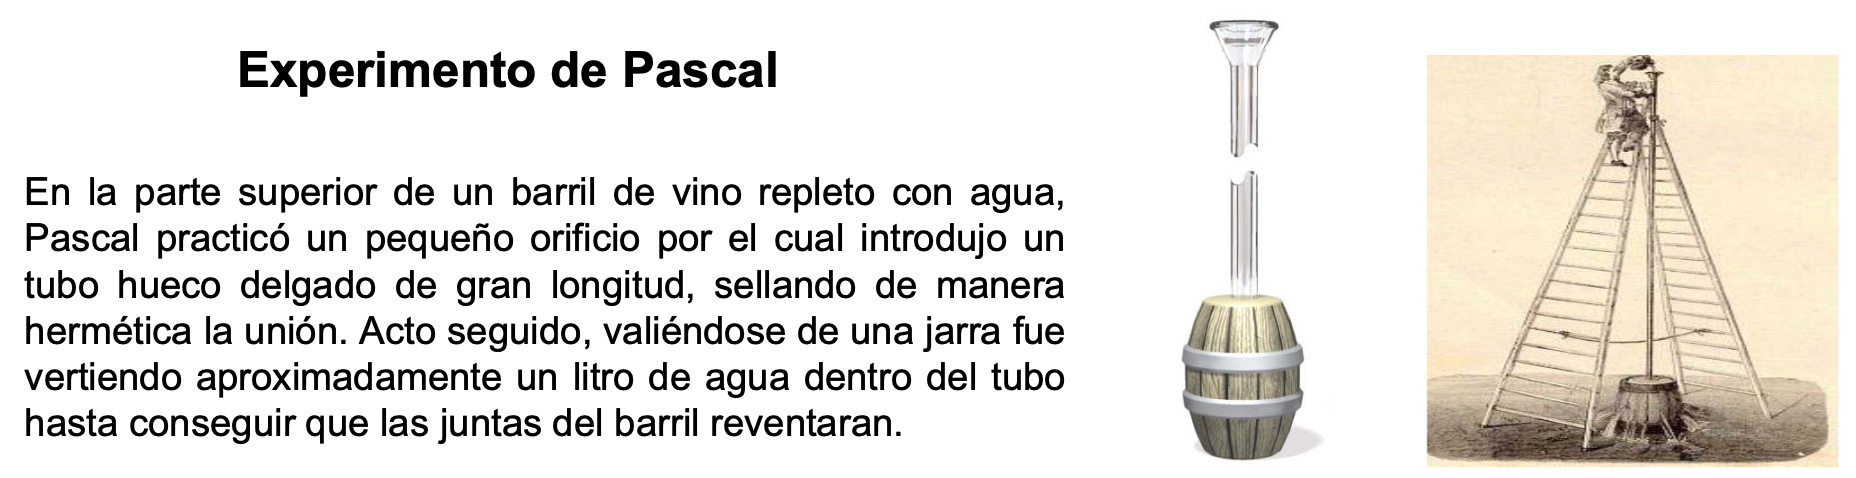
\includegraphics[width=1\textwidth]{imagenes/imagenes07/T07IM15.png}
	\caption*{El `rompetoneles' de Pascal.}
\end{figure}

\vspace{20mm} %*****************************************

\section{Principio de Arquímedes}

\emph{``Todo cuerpo sumergido en un fluido experimenta un empuje (fuerza) vertical y hacia arriba igual al peso del volumen del líquido que desaloja.''}


Tenemos el cuerpo en reposo, las fuerzas laterales se anulan. 

Veamos las fuerzas que actúan.

\vspace{20mm} %*****************************************

\begin{multicols}{2}
\begin{figure}[H]
	\centering
	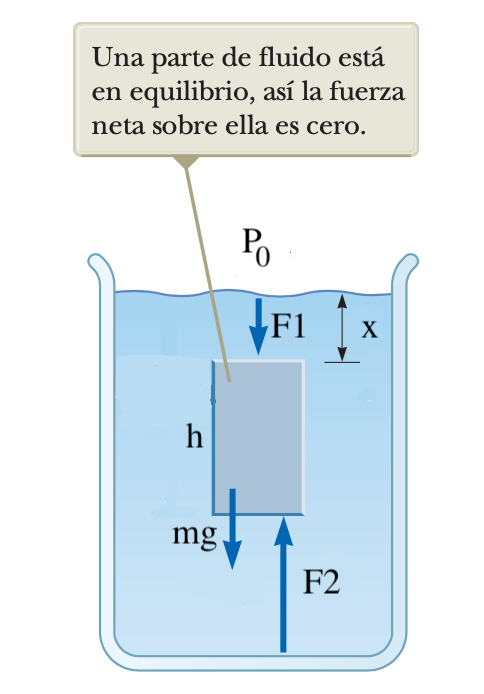
\includegraphics[width=.5\textwidth]{imagenes/imagenes07/T07IM09.png}
\end{figure}

$\quad$

$\quad$

\begin{figure}[H]
	\centering
	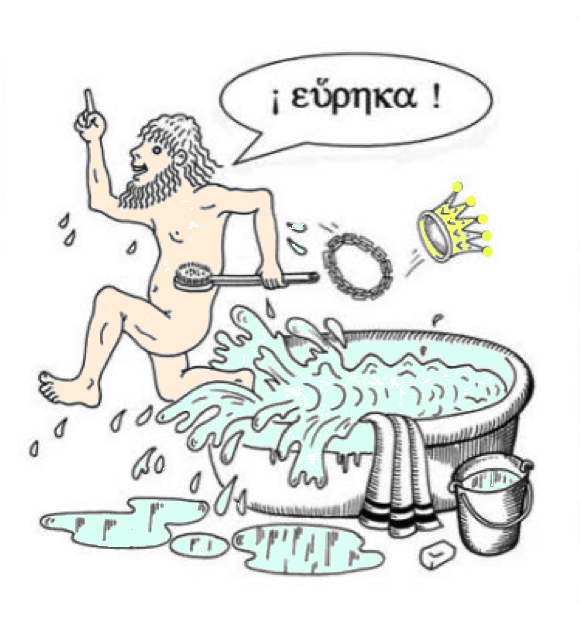
\includegraphics[width=.5\textwidth]{imagenes/imagenes07/T07IM08.png}
\end{figure}
\end{multicols}


$mg;\qquad F_1=(P_0+\rho_a g h)S; \qquad F_2=-[P_0+\rho_ag(x+h)]S$

$F_2-F_1=\rho_a g h S=g \rho_a V_{cuerpo}=g m_a$, esta es la fuerza hacia arriba que describe Arquímedes.
$F_{resultante}=mg-m_ag$, si 

$\begin{cases}\ F_R>0:\quad mg>m_ag \to \text{ haca abajo} \\ \ F_R<0:\quad mg<m_ag \to \text{ haca arriba} \end{cases}$


El principio de Arquímedes es, hoy, un teorema.


\begin{figure}[H]
	\centering
	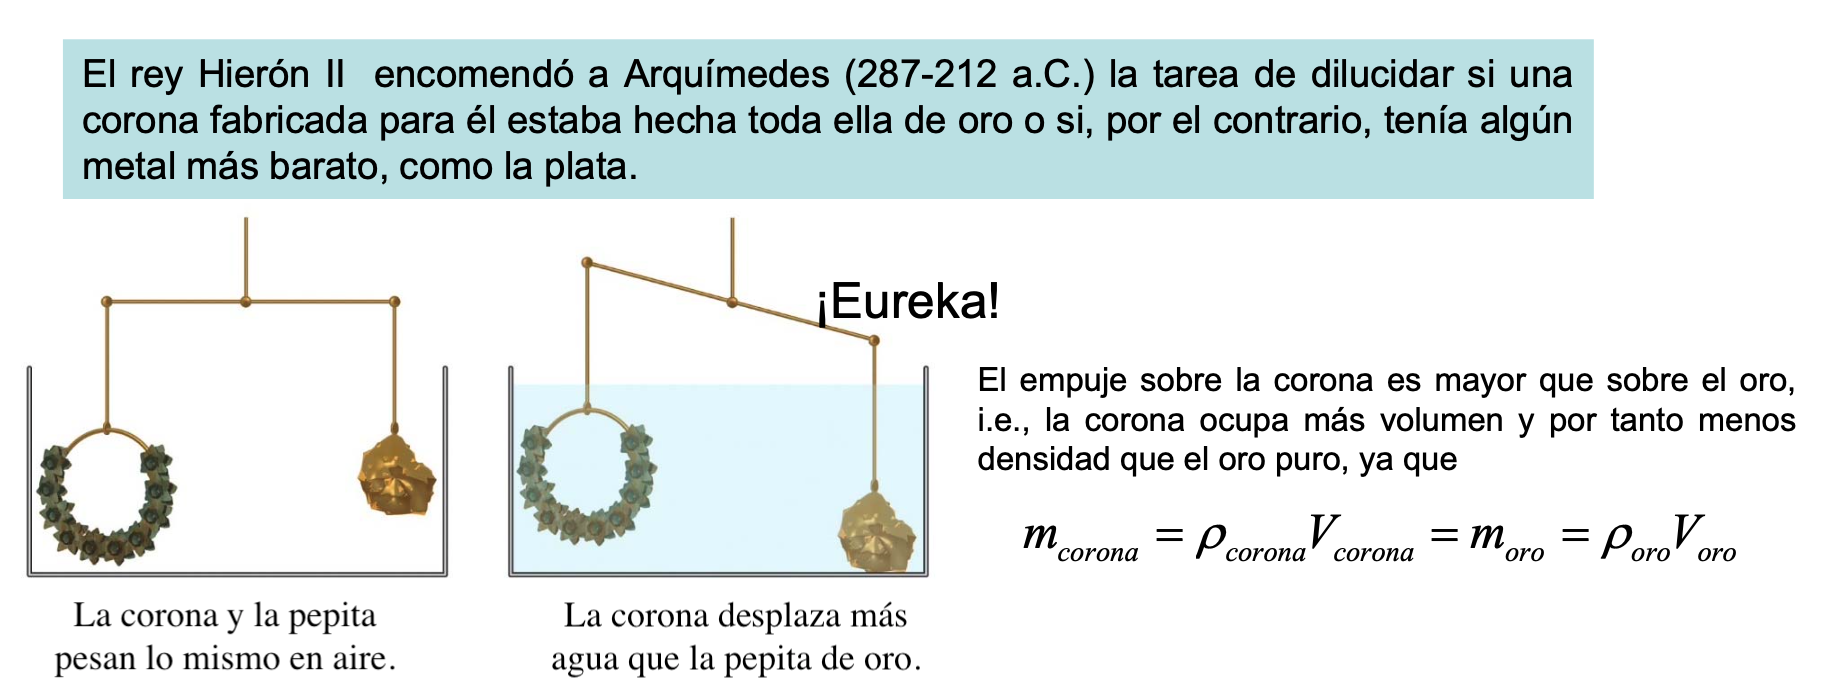
\includegraphics[width=1\textwidth]{imagenes/imagenes07/T07IM12.png}
\end{figure}

\newpage %***********************************************
\section{Fuerzas contra un dique}

\begin{multicols}{2}
A una profundidad $\ y:$ 

$P=P_0+\rho g y.\ $  

Sobre un elemento de superficie $\dd S$ del dique, la fuerza elemental resultantes será  $\dd F_R=P\dd S$.

$\begin{cases} P \ \dd S=(P_0+\rho g y)\ \dd S \\ P_0 \ \dd S \end{cases} \Rightarrow$ 

$\dd F_R= P \ \dd S=\rho g y \ \dd S =\rho g y L \ \dd y$

$\displaystyle \boldsymbol{F_R}=\int \dd F_R =\rho g L \int_0^h y \ \dd y= $ 

$=\boldsymbol{\dfrac 1 2 \rho \ g \ L \ h^2}$


\begin{figure}[H]
	\centering
	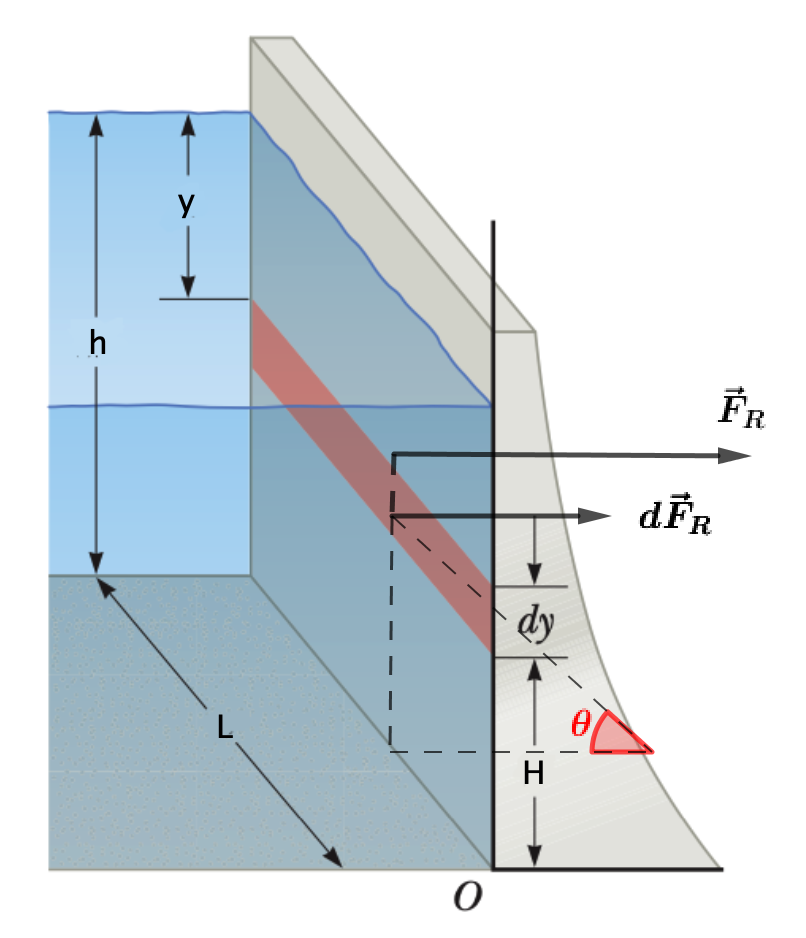
\includegraphics[width=.4\textwidth]{imagenes/imagenes07/T07IM13.png}
\end{figure}
\end{multicols}

Considerando ahora el dique como un cuerpo rígido. vamos a encontrar donde se aplica esta fuerza resultante.



$\dd \overrightarrow{M}=\vec r \times \dd \vec F_R;\quad$
$\dd M=r\  \dd F_R\  \sin \theta=$
$=(h-y) \ \dd F_r$

$M=\int (h-y)\ \dd F_R=$
$=\displaystyle \int_0^h (h-y)\ \dd r=$
$\displaystyle =\int_0^y (h-y) \rho g L y \dd y$

$\boldsymbol{M=}\displaystyle \int_0^h \rho g L h \ y \ \dd y -\int_0^h \rho g L \ y^2 \ \dd y=\dfrac{\rho g L h^3}2-\dfrac{\rho g L h^3}6 \boldsymbol{=\rho g L \dfrac {h^3}6}$

Por otra parte, $M=F_R\ H \to \quad H=\dfrac 1{F_R} \rho g L \dfrac{h^3}6=\dfrac{\rho g L h^3 / 6}{\rho g L h^2/2}=\dfrac h 3$

Luego: $\quad \boldsymbol{H=\dfrac h 3}$


\section{Problemas}

\begin{prob}
Un tubo en U sencillo contiene $Hg$. Cuando se echan $13.6\ \mathrm{cm}$ de agua en su rama derecha, ¿cuánto se eleva el mercurio en su rama izquierda a partir de su nivel original?	
\end{prob}
\begin{multicols}{2}
$P_0+\rho_{Hg}g \ x+\rho_{Hg}g\ h=$

$=P_0 + \rho_{Hg} \ x + \rho_a g \ h_a \to$

$\to \quad h=\dfrac {\rho_a}{\rho_{Hg}}\ h_a $

Con los datos del problema (buscando $\rho_a=1 \mathrm{g}\ \mathrm{cm}^{-3}; \ \rho_{Hg}=13.6 \ \mathrm{g\ cm}^{-3}$),

$h=1\ \mathrm{cm}$
\begin{figure}[H]
	\centering
	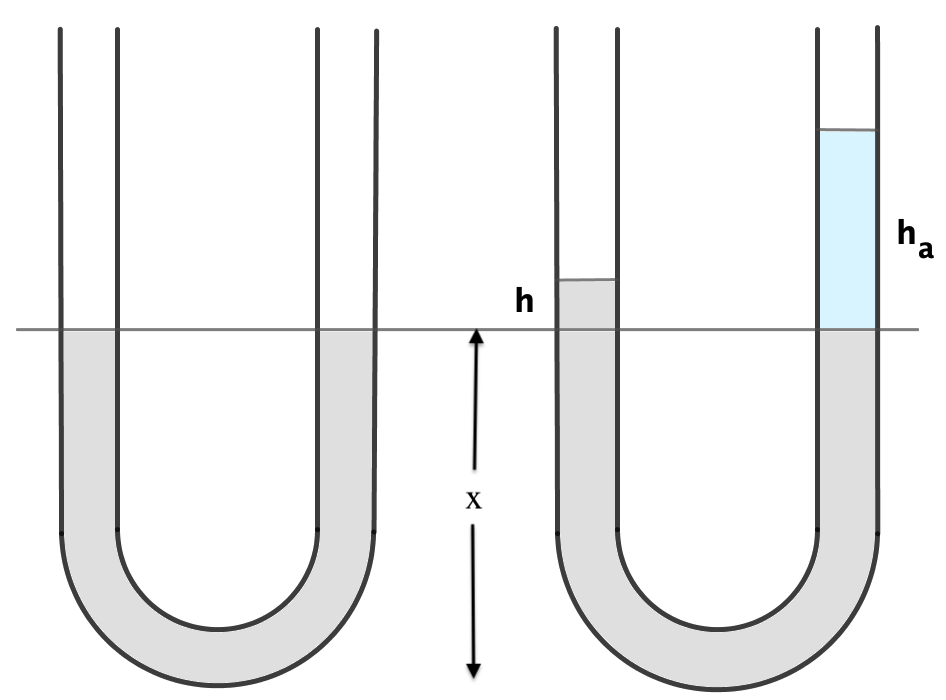
\includegraphics[width=.35\textwidth]{imagenes/imagenes07/T07IM19.png}
\end{figure}	
\end{multicols}

\vspace{30mm} %*****************************************************
\begin{prob}	
\end{prob}
\begin{figure}[H]
	\centering
	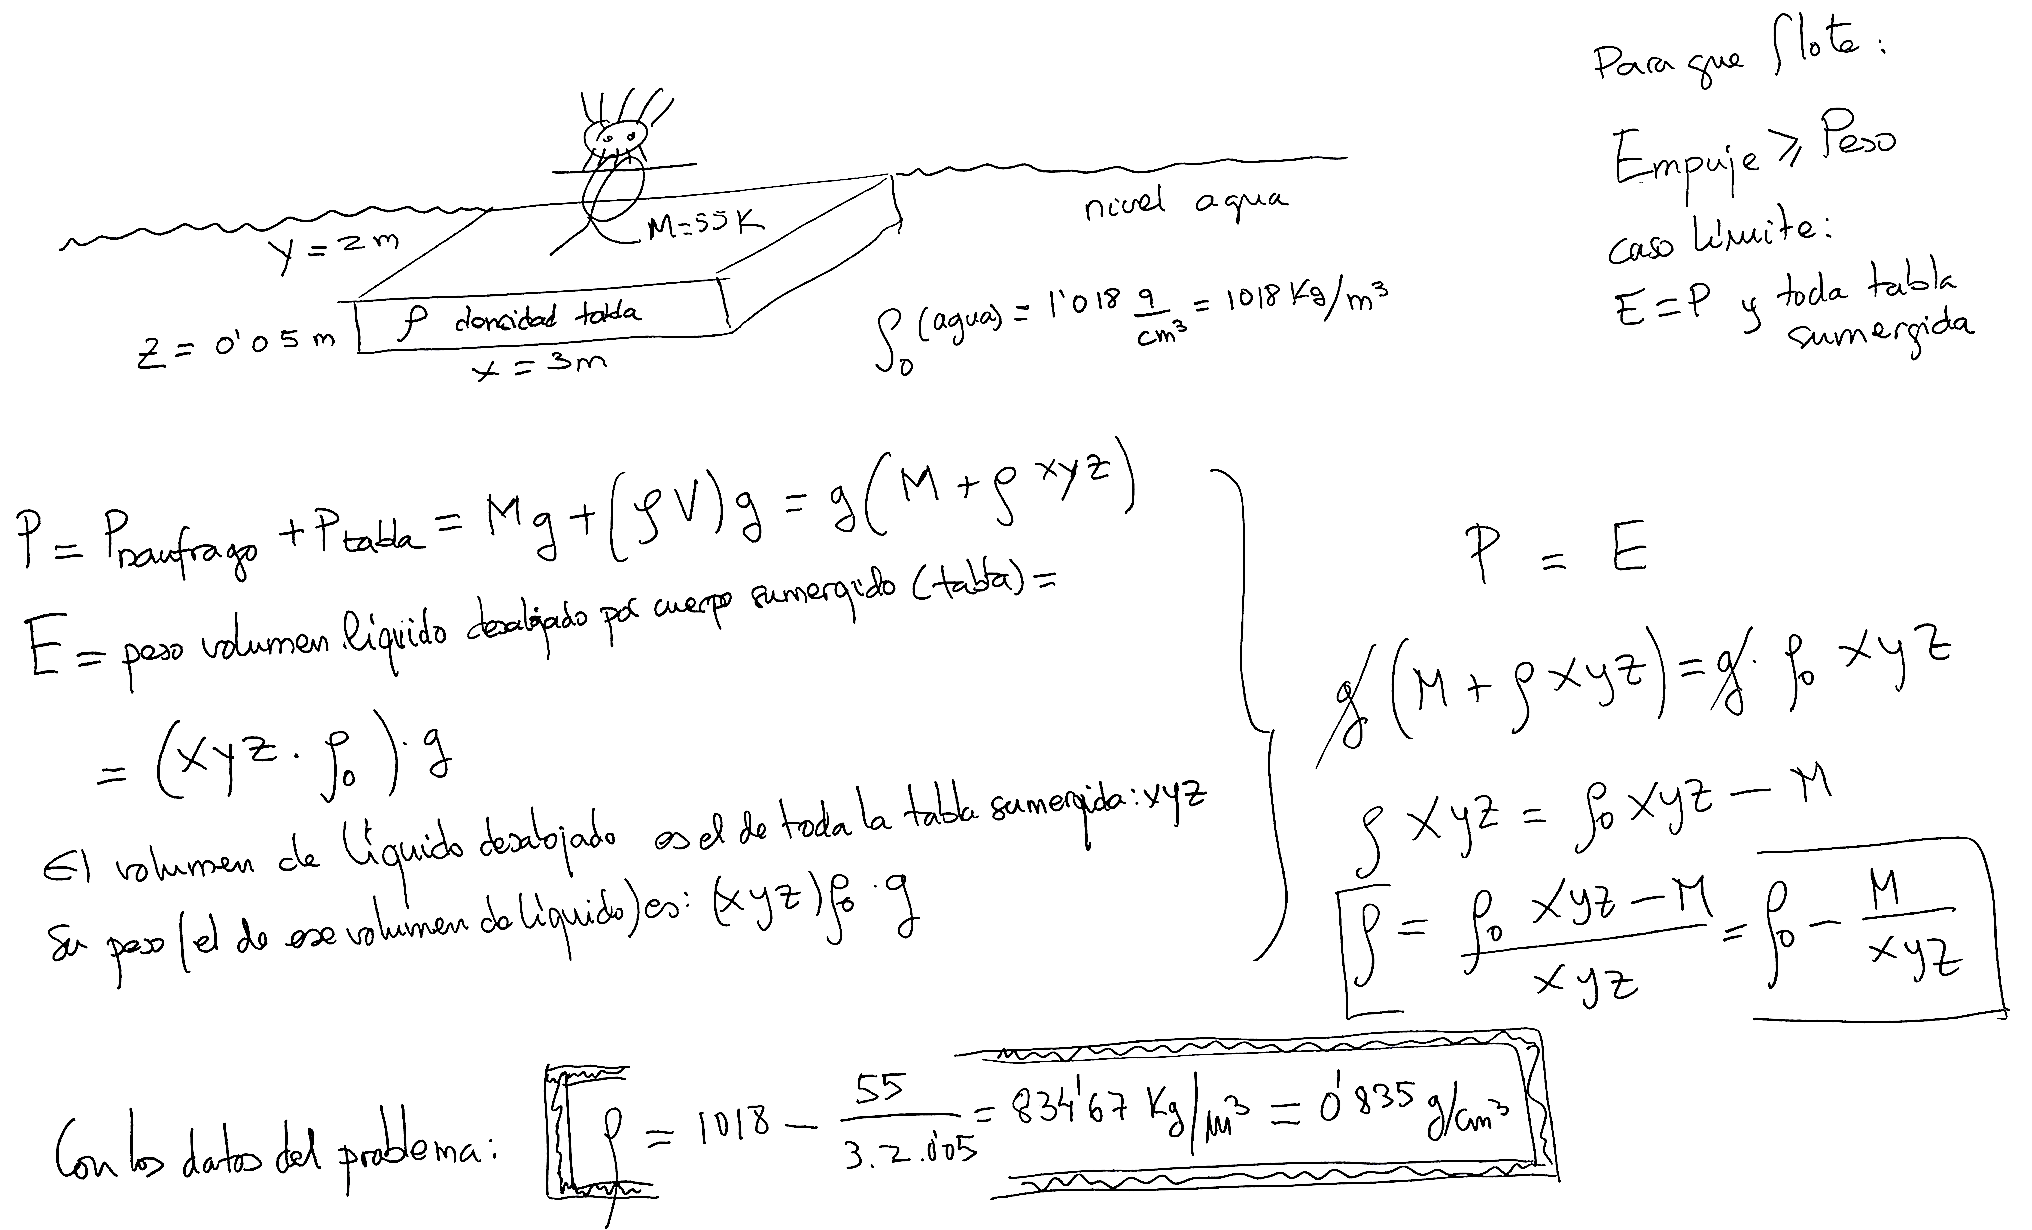
\includegraphics[width=1\textwidth]{imagenes/imagenes07/T07IM18.png}
\end{figure}



\begin{prob}
	Una plataforma flotante de área $A$ y espesor $H$ y masa $M=600\ \mathrm{kg}$ flota en agua tranquila con una inmersión de $h_0=7\ \mathrm{cm}$. Cuando una persona sube a la plataforma, la inmersión es de $h_1=8.4\ \mathrm{cm}$. ?`Cuál es la masa $m$ de la persona?
\end{prob}

\begin{multicols}{2}
Arquímedes: Peso = Empuje

Sin hombre: $Mg=Ag \rho_l \ h_0$

Con hombre: $(M+m)g=Ag \rho_l \ h_1$

Dividiendo: $\dfrac {M+m}{M}=\dfrac {h_1}{h_0}$

Luego: $m=\left( \dfrac{h_1}{h_0}-1 \right)\ M$

Datos del problema $\to m=120\ \mathrm{kg}$.
\begin{figure}[H]
	\centering
	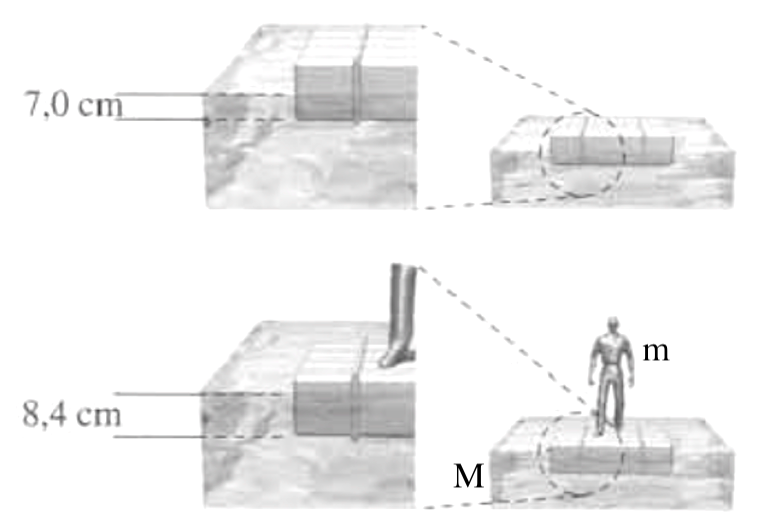
\includegraphics[width=.5\textwidth]{imagenes/imagenes07/T07IM20.png}
\end{figure}	
\end{multicols}
\begin{prob}
\begin{multicols}{2}.

Tenemos un vaso de agua en el que flota un trozo de hielo de forma que el nivel de agua llega justamente al borde del vaso. Cuando se funda el hielo, ?`aumentará el nivel de agua derramándose por el vaso, permanecerá igual, disminuirá?	
\begin{figure}[H]
	\centering
	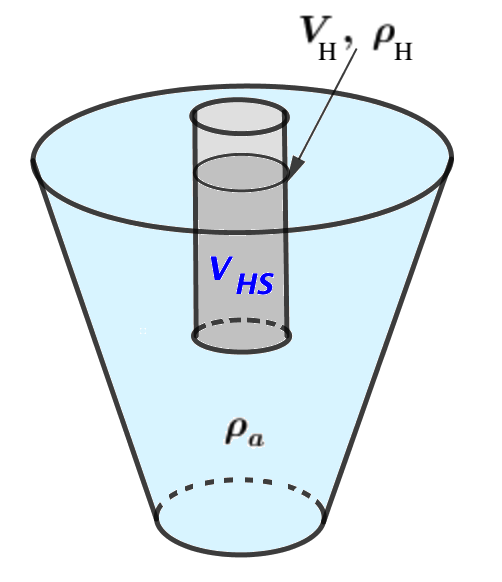
\includegraphics[width=.2\textwidth]{imagenes/imagenes07/T07IM21.png}
\end{figure}
\end{multicols}
\end{prob}

--- Inicialmente: $\ V_1=V_{agua}+V_{hielo \ sumergido}=V_a+V_{HS}$

En equilibrio, Arquímedes:  $P=E \ \to \ m_{HT}\ \rho_H g=V_{HS} \ \rho_a g$

\textcolor{gris}{Subíndices: $a=agua;\ HT=hielo\ total;\ HS=hielo\ sumergido; \ h=hielo$}

Luego: $\ V_{HT} \ \rho_h \ g=V_{HS}\ \rho_a \ g \ to \to \dfrac{V_{HS}}{V_{HT}}=\dfrac{\rho_h}{\rho_a}$

Por lo que: $\ V_1=\dfrac {m_a}{\rho_a}+\dfrac{\rho_h}{\rho_a}V_{HT}= 
\dfrac {m_a}{\rho_a}+\dfrac{\rho_h}{\rho_a}\ \dfrac{m_{HT}}{\rho_h}=
\dfrac {m_a}{\rho_a}+\dfrac{m_{HT}}{\rho_a}$

$V_1=
\dfrac{1}{\rho_a}\ (m_a+m_{HT}) \quad (1*)$

--- Cuando todo el hielo funde: $\ V_2=V_a+V_{H\to a}=\dfrac{m_a}{\rho_a}+\dfrac{m_{HT}}{\rho_h}$

$V_2=
\dfrac{1}{\rho_a}\ (m_a+m_{HT}) \quad (2*)$

--- Conclusión: como $(1*)=(2*)\ \to \ V_1=V_2 \ $ el volumen queda igual.

\begin{prob}
Dos cuerpos, iguales en forma y tamaño pero uno más denso que el otro, se sueltan simultáneamente desde una misma altura. Suponiendo que la resistencia del aire es la misma en ambos, ¿cuál de los dos llegará antes al suelo?	
\end{prob}

\begin{multicols}{2}
$F_{Tot}=mg-E-R$

$V_1=V_2;\ \ R_1=R_2;\ \ aire:\ \rho_0$

$F_1=\rho_1Vg-\rho_aVg-R=m_1a_1$

$F_2=\rho_2Vg-\rho_aVg-R=m_2a_2$

El cuerpo que caerá más rápido será aquel que posea mayor aceleración.
\begin{figure}[H]
	\centering
	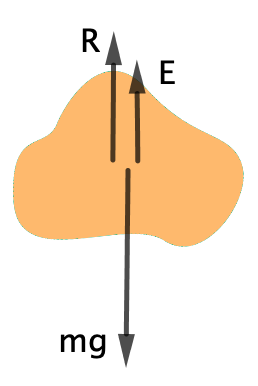
\includegraphics[width=.2\textwidth]{imagenes/imagenes07/T07IM22.png}
\end{figure}
\end{multicols}

$a_1=\dfrac{Vg(\rho_1-\rho_0)-R}{V\rho_1}=g \left( 1-\dfrac{\rho_0}{\rho_1} \right)-\dfrac{R}{V\rho_1}$

$a_2=\dfrac{Vg(\rho_2-\rho_0)-R}{V\rho_2}=g \left( 1-\dfrac{\rho_0}{\rho_2} \right)-\dfrac{R}{V\rho_2}$


--- Hipótesis: $\quad \rho_1>\rho_2\ \to \ \rho_1-\rho_2>0 $

Calculemos $\ a_1-a_2=g\left[ \dfrac{\rho_0}{\rho_2}-\dfrac{\rho_0}{\rho_1} \right]+\dfrac R V \left[ \dfrac{1}{\rho_2}-\dfrac{1}{\rho_1} \right]$

$a_1-a_2=
\dfrac{1}{\rho_1\ \rho_2} \left[ g\rho_0\ \cancelto{>0}{(\rho_1-\rho_2)}+\dfrac R V \ \cancelto{>0}{(\rho_1-\rho_2)} \right]>0$

Como $\ a_1-a_2>0 \  \to \ a_1>a_2$, por lo que la aceleración es mayor en el cuerpo más denso y cae más deprisa.


\begin{prob}
Una esfera hueca de radio interior $r_i=9\ \mathrm{cm}$ y radio exterior $r_e=10\ \mathrm{cm}$ flota en un líquido de densidad $\rho_l	= 0.8 \ \mathrm{g\ cm}^{-3}$ sumergido hasta el ecuador. 

$\ \ \ a)\quad$ ¿Cuál es la densidad de la esfera, $\rho_s$?

$\ \ \ b)\quad$ ¿Cuál debería ser la densidad del líquido para que el líquido flotase sumergido por entero?
\end{prob}

\begin{multicols}{2}
El volumen del material del que está hecha la esfera es:
$\ V_T=\frac 4 3 \pi (r_e^3-r_i^3)$

El volumen sumergido que ocupa media esfera es:
$\ V_S=\frac 1 2 \frac 4 3 \pi r_e^3$

--- a) Arquímedes: $\ V_T\rho_s g=V_S \rho_l g$
\begin{figure}[H]
	\centering
	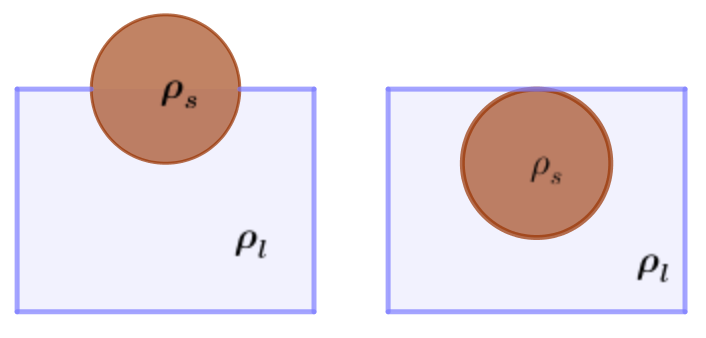
\includegraphics[width=.5\textwidth]{imagenes/imagenes07/T07IM23.png}
\end{figure}
\end{multicols}
$\rho_s = \dfrac{V_S}{V_T}\rho_l \ =1.476\ \mathrm{g\ cm}^{-3}$ 

--- b) Esfera completamente sumergida, ahora $V_S'=\frac 4 3 \pi r_e^3$

Arquímedes: $\ V_T\rho_s g=V_S' \rho_l g$

$\rho_l=\dfrac{V_T}{V_S'}\rho_S=\dfrac{r_e^3-r_i^3}{r_e^3} \rho_S=\ 0.400 \ \mathrm{g\ cm}^{-3}$ 



\begin{prob}
\begin{multicols}{2}
Un cuerpo de densidad $\rho$ se posa suavemente sobre la superficie del agua \textcolor{gris}{($\rho_0=1\ \mathrm{gcm}^{-3}$)} contenida en un recipiente y se observa que tarda en llegar al fondo un tiempo $t$. Se repite la experiencia con un cuerpo de densidad $\rho'$ que tarda un tiempo $t'$ en llegar al fondo. Calcula la expresión de $\rho'$ y su valor numérico cuando $\rho=1.6 \ \mathrm{gcm}^{-3}$ y $t'=2t$.
\begin{figure}[H]
	\centering
	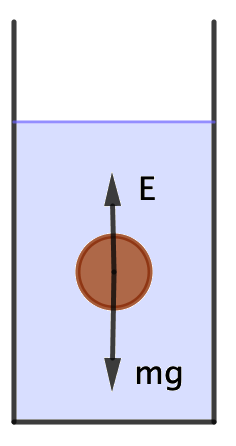
\includegraphics[width=.15\textwidth]{imagenes/imagenes09/T09IM10.png}
\end{figure}	
\end{multicols}
\end{prob}


$F_{Total}=mg-E=\rho g V-\rho_0gV=(\rho-\rho_0)Vg=ma=\rho V a \to $

$\boldsymbol{ a=\dfrac{\rho-\rho_0}{\rho}\ g}$; $\ a=cte:\ \ MRUA$

$H=0+0+\frac 1 2 a t^2=\frac 1 2 \dfrac{\rho-\rho_0}\rho g \ t^2 
\to$
$\quad \boldsymbol{ t=\sqrt{\dfrac {2H}{g}\ \dfrac{\rho}{\rho-\rho_0}} }$


Para el otro cuerpo: $\quad \boldsymbol{a=\dfrac{\rho'-\rho_0}{\rho'}\ g} ; \qquad \boldsymbol{t'=\sqrt{\dfrac {2H}{g}\ \dfrac{\rho'}{\rho'-\rho_0}}}$

Puesto que los dos cuerpos recorren la misma distancia $H$:

$\frac 1 2 \dfrac{\rho-\rho_0}\rho g \ {t}^2=
\frac 1 2 \dfrac{\rho'-\rho_0}\rho' g \ {t'}^2 \to $
$\ 1-\dfrac {\rho_0}{\rho'}=1-\left[\dfrac{\rho-\rho_0}{\rho} \ \left(\dfrac{t}{t'} \right)^2\right] \to \ $

$\boxed{\rho'=\dfrac{\rho}{1-\left[\dfrac{\rho-\rho_0}{\rho} \ \left(\dfrac{t}{t'} \right)^2\right]}}$

Con los datos del problema, $\rho=1.6;\ \rho_0=1;\ t'=2t \to \ \ \rho'=1.766\ \mathrm{gcm}^{-3}$


\newpage %************************************

\begin{myblock}{La paradoja hidrostática}
Fíjate en estos tres recipientes. Los tres tienen una base circular de $10\ \mathrm{cm}$ de diámetro y están llenos de agua hasta una altura de $20\ \mathrm{cm}$. El agua ejerce una presión, la presión hidrostática, sobre el fondo de cada recipiente.\footnote{https:semillasdelaciencia.weebly.com/la-paradoja-hidrostaacutetica.html}

\begin{figure}[H]
	\centering
	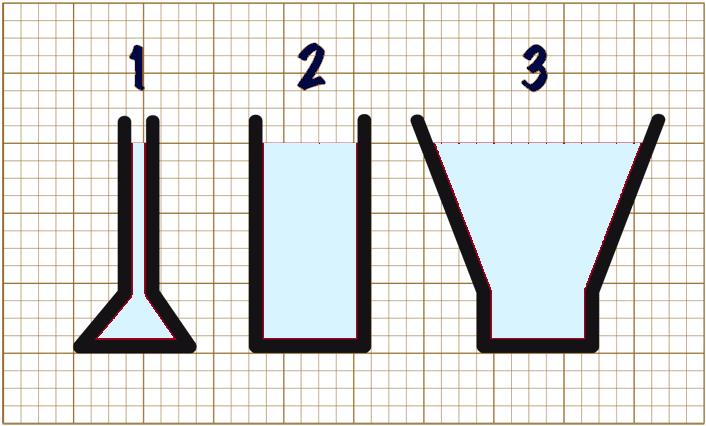
\includegraphics[width=.75\textwidth]{imagenes/imagenes07/T07IM24.png}
\end{figure}
	\emph{?`Cuál de los tres recipientes soporta una mayor fuerza en el fondo?}
	
	Parece razonable pensar que el tercer recipiente, que contiene más agua, será el que soporte más fuerza en el fondo, pero $\cdots$
	
	Calculemos la fuerza sobre el fondo de cada uno de los tres recipientes:

--- i) Calculamos la presión hidrostática $(P=\rho g h)$ en el fondo de cada recipiente.

--- ii) Calculamos el área del fondo de cada recipiente $(S=\pi r^2)$.

--- iii) Como la presión es fuerza entre superficie $(P=F/S)$, calculamos la fuerza multiplicando la presión por la superficie $(F=P\ S)$.
\begin{figure}[H]
	\centering
	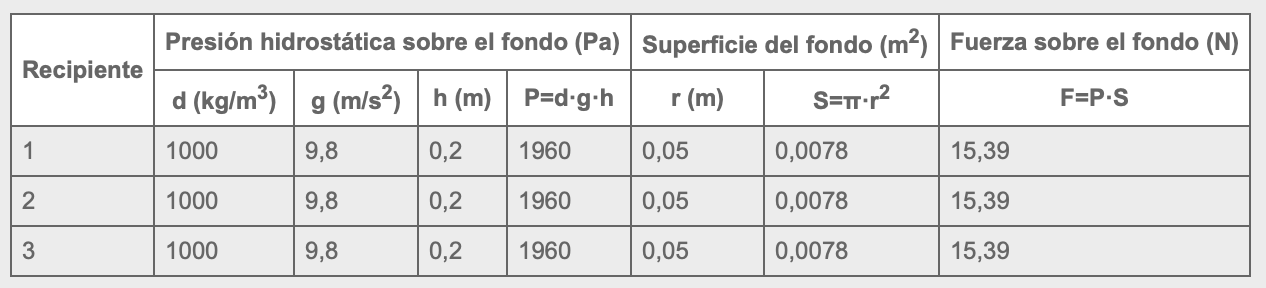
\includegraphics[width=1\textwidth]{imagenes/imagenes07/T07IM25.png}
\end{figure}

\emph{!`La fuerza que ejerce el agua sobre el fondo es la misma en los tres recipientes, independientemente de la cantidad de agua que contienen!}

Como los tres recipientes están llenos del mismo líquido hasta la misma altura, la presión hidrostática en el fondo es igual para todos. En consecuencia, al tener todos la misma base, la fuerza sobre el fondo será idéntica, independientemente de la cantidad de líquido que contengan. Este hecho, que parece estar en contradicción con el sentido común, recibe el nombre de \emph{\textbf{paradoja hidrostática}}\footnote{Según la RAE, una \emph{paradoja} es una ``idea extraña u opuesta a la común opinión y al sentir de las persona.''}

\vspace{4mm}
 
 \rule{100pt}{0.2pt}

\vspace{4mm}
La fuerza debida a la presión que ejerce un fluido en la base de un recipiente puede ser mayor o menor que el peso del líquido que contiene el recipiente, esta es en esencia la paradoja hidrostática.

\vspace{4mm}
\textbf{Recipiente de forma cónica.}\footnote{http://www.sc.ehu.es/sbweb/fisica/fluidos/estatica/paradoja/paradoja.htm}

\vspace{2mm} Sea un recipiente en forma cónica, de altura $h$, cuya base tiene un radio $R$ y que está completamente lleno de líquido.

\begin{figure}[H]
	\centering
	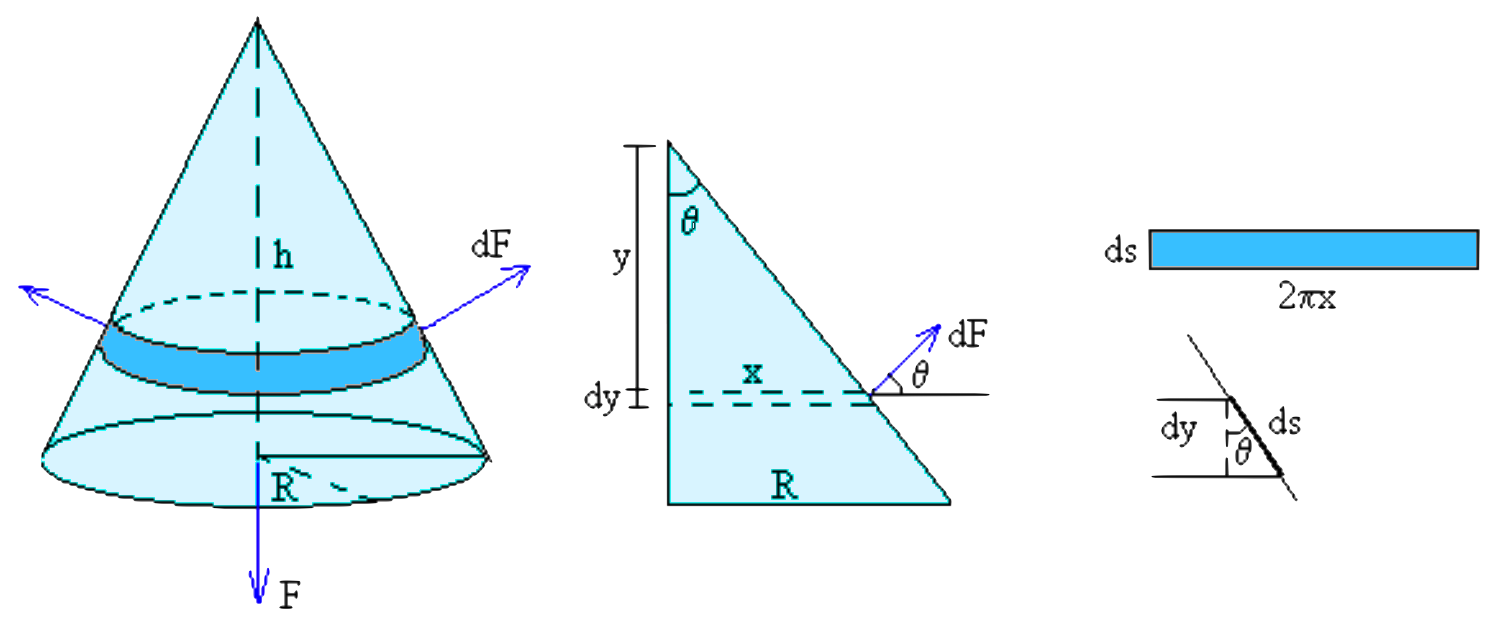
\includegraphics[width=1\textwidth]{imagenes/imagenes07/T07IM26.png}
\end{figure}

\vspace{2mm} El peso del líquido de densidad $\rho$ es $mg=\rho V_{cono} g=\rho \frac 1 3 \pi R^2 h g$

\vspace{2mm} La fuerza hacia abajo que ejerce el líquido en su base debido a la presión es $F=P\ S=\rho g h \pi R^2$, que es el triple del peso del líquido contenido en el cono $(F=3mg)$.

\vspace{2mm} La solución de esta aparente paradoja está en considerar todas las fuerzas que ejerce el líquido debido a la presión en la superficie cónica y que son perpendiculares a la misma.



\vspace{2mm} La fuerza $\dd F$ que ejerce el líquido sobre el elemento de la superficie cónica comprendido entre $y$ e $ y+ \dd y$ es el producto de la presión del líquido a la profundidad $y$, multiplicado por el área de la superficie del tronco de cono de radio $x$ y altura $\dd y$. El área de esta superficie es equivalente a la de un rectángulo de longitud $2\pi x$  y anchura $\dd s=\dd y / \cos \theta$.

\vspace{2mm} La fuerza es $\dd F=\rho g y \cdot 2 \pi x \dd s$

\vspace{2mm} La componente vertical de dicha fuerza es $\dd F_y= \dd F \cdot \sin \theta= \rho g y \cdot 2 \pi x \dd y \cdot \tan \theta$, que apunta hacia arriba (signo menos, por convenio).

\vspace{2mm} Como la relación entre $x $ e $y$  y el ángulo $\theta$  es  $\tan \theta=R/h$, la componente vertical de la suma de todas las fuerzas que ejerce el líquido sobre los elementos de la superficie lateral del cono será:

\vspace{2mm} $F_y=\displaystyle \dfrac{2 \pi \rho g R^2}{h^2} \int_0^h y^2 \dd y = \dfrac 2 3 \pi \rho g r^3 h$

\vspace{2mm} Finalmente, la componente vertical de la resultante de las fuerzas que ejerce el líquido debido a la presión sobre superficie total del cono es


$F-F_y=\rho g \pi R^2 h-\dfrac 2 3 \rho g \pi R^2 h=\dfrac 1 3 \rho g \pi R^2 h$,
que está dirigida hacia abajo, y coincide con el peso del fluido.

\vspace{2mm} Como hemos comprobado, la paradoja hidrostática consiste en que la fuerza debida a la presión del líquido sobre la base del recipiente puede ser diferente del peso del líquido que lo contiene, paradoja que se resuelve en el momento en el que consideramos las componentes verticales de las fuerzas que ejerce el líquido sobre todas las paredes del recipiente originadas por la la presión.

\end{myblock}




